\vspace{-2ex}\makebox[0in][l]{\Large\textsf{Empowering faculty to run online learning experiments}}
\vspace{1ex}

\begin{sectionblock}{A Solution}
  This project collects and analyzes student interaction data through
  a distributed educational technology framework weaving together
  authors, instructors, researchers, and learners.

  \vspace{1ex}We call the platform \textbf{the Distributed Open
    Education Network}, or Doenet.  In short, Doenet measures student
  interactions with web pages and stores anonymized data in an open
  and distributed data warehouse.
\end{sectionblock}

\vspace{1ex}

\begin{sectionblock}{Built around Interactivity}

  \begin{wrapfigure}{R}{0.5\textwidth}
    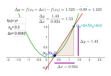
\includegraphics[width=0.48\textwidth]{math-insight.pdf}
  \end{wrapfigure}
  We investigate the benefits of virtual manipulatives and the
  influence of the support given to learners as they navigate online
  activities.

  \vspace{1ex}The event log resides in an open data warehouse, so 
  educational researchers can probe the data to generate additional
  knowledge on student learning.
\end{sectionblock}

    
